\documentclass[11pt,a4paper,twoside,f1,ngerman]{HsH-report}

\usepackage{color}
\usepackage{lipsum}
\usepackage{siunitx}
\usepackage{biblatex}
\addbibresource{src/localBibliography.bib}

\begin{document}


\pagenumbering{Roman}
\maketitle
\declarationAuthorship

\begin{abstract}
	\lipsum[5-8]
\end{abstract}

\tableofcontents

\cleardoublepage % unbedingt erforderlich bei Doppelseitigem layout vor neuer Seitennummerierung!
\pagenumbering{arabic} % Seitennummerierung normale zahlen

\chapter{one}
	\label{chap: one}
	{\color{red}test} und stuff
	\begin{figure}
		\centering
		
\includegraphics[width=.6\textwidth]{img/lorem-ipsum.jpg}
		\caption{test}
	\end{figure}

	noch ein test \normalsubscripts$R_t$ \upsubscripts$R_t$

	mit einheit: $R=200\,\milli\ohm+ \SI{0.34567453}{\volt\per\metre}$
	\cite{laboranleitung:physik}
	\vspace{2cm}\\\pagebreak
	eine zahl: $3,5+3.5$\\

	\begin{figure}
		\centering
		\includegraphics[width=0.6\textwidth, page=2]{plt/build/examplePlot.pdf}
		\caption{a nice plot}
	\end{figure}

	\begin{figure}
		\centering
		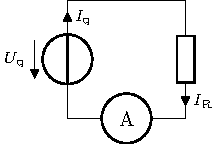
\includegraphics{img/build/exampleCircuit.pdf}
		\caption{a circuit diagramm}
	\end{figure}

	\begin{figure}
		\centering
		\graphicspath{{img/build/}} % double curly brackets needet for unknown reason
		\input{img/build/exampleSVG.pdf_tex}
		\caption{made via inkscape}
	\end{figure}

\printbibliography
\listoffigures
\end{document}
